% Options for packages loaded elsewhere
\PassOptionsToPackage{unicode}{hyperref}
\PassOptionsToPackage{hyphens}{url}
%
\documentclass[
  english,
  man]{apa6}
\title{Who does big team science?}
\author{Erin M. Buchanan\textsuperscript{1} \& Savannah C. Lewis\textsuperscript{2}}
\date{}

\usepackage{amsmath,amssymb}
\usepackage{lmodern}
\usepackage{iftex}
\ifPDFTeX
  \usepackage[T1]{fontenc}
  \usepackage[utf8]{inputenc}
  \usepackage{textcomp} % provide euro and other symbols
\else % if luatex or xetex
  \usepackage{unicode-math}
  \defaultfontfeatures{Scale=MatchLowercase}
  \defaultfontfeatures[\rmfamily]{Ligatures=TeX,Scale=1}
\fi
% Use upquote if available, for straight quotes in verbatim environments
\IfFileExists{upquote.sty}{\usepackage{upquote}}{}
\IfFileExists{microtype.sty}{% use microtype if available
  \usepackage[]{microtype}
  \UseMicrotypeSet[protrusion]{basicmath} % disable protrusion for tt fonts
}{}
\makeatletter
\@ifundefined{KOMAClassName}{% if non-KOMA class
  \IfFileExists{parskip.sty}{%
    \usepackage{parskip}
  }{% else
    \setlength{\parindent}{0pt}
    \setlength{\parskip}{6pt plus 2pt minus 1pt}}
}{% if KOMA class
  \KOMAoptions{parskip=half}}
\makeatother
\usepackage{xcolor}
\IfFileExists{xurl.sty}{\usepackage{xurl}}{} % add URL line breaks if available
\IfFileExists{bookmark.sty}{\usepackage{bookmark}}{\usepackage{hyperref}}
\hypersetup{
  pdftitle={Who does big team science?},
  pdfauthor={Erin M. Buchanan1 \& Savannah C. Lewis2},
  pdflang={en-EN},
  pdfkeywords={big team, science, authorship, credit},
  hidelinks,
  pdfcreator={LaTeX via pandoc}}
\urlstyle{same} % disable monospaced font for URLs
\usepackage{graphicx}
\makeatletter
\def\maxwidth{\ifdim\Gin@nat@width>\linewidth\linewidth\else\Gin@nat@width\fi}
\def\maxheight{\ifdim\Gin@nat@height>\textheight\textheight\else\Gin@nat@height\fi}
\makeatother
% Scale images if necessary, so that they will not overflow the page
% margins by default, and it is still possible to overwrite the defaults
% using explicit options in \includegraphics[width, height, ...]{}
\setkeys{Gin}{width=\maxwidth,height=\maxheight,keepaspectratio}
% Set default figure placement to htbp
\makeatletter
\def\fps@figure{htbp}
\makeatother
\setlength{\emergencystretch}{3em} % prevent overfull lines
\providecommand{\tightlist}{%
  \setlength{\itemsep}{0pt}\setlength{\parskip}{0pt}}
\setcounter{secnumdepth}{-\maxdimen} % remove section numbering
% Make \paragraph and \subparagraph free-standing
\ifx\paragraph\undefined\else
  \let\oldparagraph\paragraph
  \renewcommand{\paragraph}[1]{\oldparagraph{#1}\mbox{}}
\fi
\ifx\subparagraph\undefined\else
  \let\oldsubparagraph\subparagraph
  \renewcommand{\subparagraph}[1]{\oldsubparagraph{#1}\mbox{}}
\fi
\newlength{\cslhangindent}
\setlength{\cslhangindent}{1.5em}
\newlength{\csllabelwidth}
\setlength{\csllabelwidth}{3em}
\newlength{\cslentryspacingunit} % times entry-spacing
\setlength{\cslentryspacingunit}{\parskip}
\newenvironment{CSLReferences}[2] % #1 hanging-ident, #2 entry spacing
 {% don't indent paragraphs
  \setlength{\parindent}{0pt}
  % turn on hanging indent if param 1 is 1
  \ifodd #1
  \let\oldpar\par
  \def\par{\hangindent=\cslhangindent\oldpar}
  \fi
  % set entry spacing
  \setlength{\parskip}{#2\cslentryspacingunit}
 }%
 {}
\usepackage{calc}
\newcommand{\CSLBlock}[1]{#1\hfill\break}
\newcommand{\CSLLeftMargin}[1]{\parbox[t]{\csllabelwidth}{#1}}
\newcommand{\CSLRightInline}[1]{\parbox[t]{\linewidth - \csllabelwidth}{#1}\break}
\newcommand{\CSLIndent}[1]{\hspace{\cslhangindent}#1}
% Manuscript styling
\usepackage{upgreek}
\captionsetup{font=singlespacing,justification=justified}

% Table formatting
\usepackage{longtable}
\usepackage{lscape}
% \usepackage[counterclockwise]{rotating}   % Landscape page setup for large tables
\usepackage{multirow}		% Table styling
\usepackage{tabularx}		% Control Column width
\usepackage[flushleft]{threeparttable}	% Allows for three part tables with a specified notes section
\usepackage{threeparttablex}            % Lets threeparttable work with longtable

% Create new environments so endfloat can handle them
% \newenvironment{ltable}
%   {\begin{landscape}\centering\begin{threeparttable}}
%   {\end{threeparttable}\end{landscape}}
\newenvironment{lltable}{\begin{landscape}\centering\begin{ThreePartTable}}{\end{ThreePartTable}\end{landscape}}

% Enables adjusting longtable caption width to table width
% Solution found at http://golatex.de/longtable-mit-caption-so-breit-wie-die-tabelle-t15767.html
\makeatletter
\newcommand\LastLTentrywidth{1em}
\newlength\longtablewidth
\setlength{\longtablewidth}{1in}
\newcommand{\getlongtablewidth}{\begingroup \ifcsname LT@\roman{LT@tables}\endcsname \global\longtablewidth=0pt \renewcommand{\LT@entry}[2]{\global\advance\longtablewidth by ##2\relax\gdef\LastLTentrywidth{##2}}\@nameuse{LT@\roman{LT@tables}} \fi \endgroup}

% \setlength{\parindent}{0.5in}
% \setlength{\parskip}{0pt plus 0pt minus 0pt}

% \usepackage{etoolbox}
\makeatletter
\patchcmd{\HyOrg@maketitle}
  {\section{\normalfont\normalsize\abstractname}}
  {\section*{\normalfont\normalsize\abstractname}}
  {}{\typeout{Failed to patch abstract.}}
\patchcmd{\HyOrg@maketitle}
  {\section{\protect\normalfont{\@title}}}
  {\section*{\protect\normalfont{\@title}}}
  {}{\typeout{Failed to patch title.}}
\makeatother
\shorttitle{Big Team Science}
\keywords{big team, science, authorship, credit\newline\indent Word count: X}
\DeclareDelayedFloatFlavor{ThreePartTable}{table}
\DeclareDelayedFloatFlavor{lltable}{table}
\DeclareDelayedFloatFlavor*{longtable}{table}
\makeatletter
\renewcommand{\efloat@iwrite}[1]{\immediate\expandafter\protected@write\csname efloat@post#1\endcsname{}}
\makeatother
\usepackage{lineno}

\linenumbers
\usepackage{csquotes}
\ifXeTeX
  % Load polyglossia as late as possible: uses bidi with RTL langages (e.g. Hebrew, Arabic)
  \usepackage{polyglossia}
  \setmainlanguage[]{english}
\else
  \usepackage[main=english]{babel}
% get rid of language-specific shorthands (see #6817):
\let\LanguageShortHands\languageshorthands
\def\languageshorthands#1{}
\fi
\ifLuaTeX
  \usepackage{selnolig}  % disable illegal ligatures
\fi


\authornote{

Erin M. Buchanan is a Professor of Cognitive Analytics at Harrisburg University of Science and Technology. Savannah C. Lewis is a graduate student at the University of Alabama.

Thank you to Dwayne Lieck for providing an extensive list of large scale projects for this manuscript.

The authors made the following contributions. Erin M. Buchanan: Conceptualization, Data curation, Formal Analysis, Methodology, Project administration, Visualization, Writing -- original draft, Writing -- review \& editing; Savannah C. Lewis: Conceptualization, Data curation, Methodology, Project administration, Writing -- original draft, Writing -- review \& editing.

Correspondence concerning this article should be addressed to Erin M. Buchanan, 326 Market St., Harrisburg, PA 17101. E-mail: \href{mailto:ebuchanan@harrisburgu.edu}{\nolinkurl{ebuchanan@harrisburgu.edu}}

}

\affiliation{\vspace{0.5cm}\textsuperscript{1} Harrisburg University of Science and Technology\\\textsuperscript{2} University of Alabama}

\abstract{
One or two sentences providing a \textbf{basic introduction} to the field, comprehensible to a scientist in any discipline.

Two to three sentences of \textbf{more detailed background}, comprehensible to scientists in related disciplines.

One sentence clearly stating the \textbf{general problem} being addressed by this particular study.

One sentence summarizing the main result (with the words ``\textbf{here we show}'' or their equivalent).

Two or three sentences explaining what the \textbf{main result} reveals in direct comparison to what was thought to be the case previously, or how the main result adds to previous knowledge.

One or two sentences to put the results into a more \textbf{general context}.

Two or three sentences to provide a \textbf{broader perspective}, readily comprehensible to a scientist in any discipline.
}



\begin{document}
\maketitle

The introduction will go here. Here's an outline:

\begin{itemize}
\item
  Big Team Science

  \begin{itemize}
  \tightlist
  \item
    one off papers
  \item
    collaborative teams
  \end{itemize}
\item
  Credibility revolution
\item
  WEIRD
\item
  \ldots{} more tbd, brain isn't braining
\item
  Research Question 1: What journals publish big team science papers?
\item
  Research Question 2: What are the types of articles that are being published in big team science?
\item
  Research Question 3: Who is involved in big team science?
\end{itemize}

For each of these research questions, we will examine the overall results of all big team research projects, and examine for change in result trends across years of publication.

\hypertarget{method}{%
\section{Method}\label{method}}

\hypertarget{studies}{%
\subsection{Studies}\label{studies}}

We defined \textbf{big team science publications} as publications with at least 10 authors that were published in peer-reviewed journals or had posted a full paper pre-print for publication review. We specifically focused on social science research, primarily \emph{psychology} for this manuscript. First, we added all known publications from collaborative teams, such as the PSA, Many Labs, and Many Babies. We examined journals that frequently publish registered replication reports (i.e., \emph{Advances in Methods and Practices in Psychological Science}) for additional publications with at least 10 authors. From these manuscripts, we identified common authors who frequently participate in these studies, and examined their Google Scholar or Open Researcher and Contributor IDentifier (ORCID) page for other publications. We reached out to social networks on Twitter to identify other publications. Last, we used Google Scholar and EBSCO to search for large projects using the following search terms: collaboration, multicultural, large scale, and big team science.

\hypertarget{data-curation}{%
\subsection{Data Curation}\label{data-curation}}

\hypertarget{rq1-journal-information}{%
\subsubsection{RQ1: Journal Information}\label{rq1-journal-information}}

Using these criteria, we identified 70 articles for inclusion on this manuscript. The publication dates on these articles ranged from 2013 to 2022, and we used the pre-print last updated date as the publication date for those articles. The current impact factor (i.e., 2022) for each journal was found on the journal page and included for journal statistics.

\hypertarget{rq2-article-information}{%
\subsubsection{RQ2: Article Information}\label{rq2-article-information}}

For each publication, we coded the list of keywords into broad labels for areas of social science (i.e., Social Psychology, Cognitive Psychology). In this section, we elected to code each article with only one main research area. Research is often cross-disciplinary, however, for simplicity, we applied one global label to each article that represented the perceived main area of study (based on what course this material might be taught in, the publication journal focus). The list of broad areas includes clinical, cognitive, developmental, educational, and social psychology. Last, we included a metascience category that covered articles that were detailing the science of science. The Open Science Collaboration {[}CITE{]} was included in this category because the aim of the paper was a focus on replication across multiple field types. Other metascience categories included papers that focused on research degrees of freedom, analysis choices, and types of samples.

\hypertarget{rq3-author-information}{%
\subsubsection{RQ3: Author Information}\label{rq3-author-information}}

The author list was then extracted from each publication. In the case of consortium authorship, we extracted the complete authorship from the meta-data or pre-print publication. The total number of unique authors was 3336. The number of authors on each publication ranged from 1 to 482 with an average of 68.63 authors (\emph{SD} = 89.89).

Next, we matched each author to their Google Scholar and ORCID profile pages, if available. We originally used the \emph{R} packages, \emph{rorcid} {[}CITE{]} and \emph{scholar} {[}CITE{]} to try to match published author names to profile pages. This process did not result in a large number of matches, and we therefore curated the list of profile pages manually, checking each author against the publication list. We used these two packages and profile pages to collect authorship statistics described below.

\textbf{\emph{Career Length}}. Career length for each author was defined using multiple variables to see if results from the two data sources would converge on similar answers. Both ORCID and Google Scholar provide a list of publications for authors, and we first calculated career length as the year of first publication listed for each author. In ORCID, a researcher can enter their educational background with completion years for each degree. We defined career length for this variable as years since first degree listed. Publication years are often curated directly from meta-data provided by Crossref (ORCID) or online sources used by Google Scholar. Authors may also directly add publications and their information into both systems. The limitation to using education as a metric for career length is that the researcher must directly enter this information into ORCID.

\textbf{\emph{Employment}}. Employment information was collected from self-entered ORCID data. These values are open text, and therefore, we coded them into coherent categories for traditional educational (graduate student, post doctoral, lecturer), tenure track (assistant, associate, full professor), and other roles (fellow, research assistant, researcher, head). Employment geopolitical region was also selected when available.

\textbf{\emph{Education}}. As with employment information, we also collected education information from self-entered ORCID data. These values were coded into general categories of bachelor, master, and doctoral degrees. The geopolitical region of the listed education was included when available. For analyses, both employment and education levels were grouped into United Nation regions.

\textbf{\emph{Types of Publications}}. ORCID includes information about the type of publication pulled from either researcher entered data or Crossref. We coded these publications into general categories including book, conference presentations, data-sets, journal articles, preprints, software, thesis, and other publications.

\textbf{\emph{Publication Metrics}}. We calculated total number of publications of any type from both Google Scholar and ORCID. We additionally pulled both the h-index and i-10 index from Google Scholar. The h-index represents the highest \emph{h} number of publications that have at least \emph{h} citations, while the i-10 index represents the number of publications with at least 10 citations.

\hypertarget{data-analysis}{%
\subsection{Data analysis}\label{data-analysis}}

\hypertarget{rq1-journals}{%
\subsubsection{RQ1: Journals}\label{rq1-journals}}

<<<<<<< Updated upstream
Behavior research method 2020
2 year 6.242
5 year 6.277

Collabra: psychology 
2 year 3.02
5year 3.296

Computers in human behavior
2 6.829
5 8.582
=======
Results for types of journals will include a summary of the journals that publish big-team science papers and an average of the 2-year and 5-year impact factors for the journals.

\hypertarget{rq2-articles}{%
\subsubsection{RQ2: Articles}\label{rq2-articles}}

Results for types of articles will include a summary of the coded areas for each article, presented overall and across the years of publication.
>>>>>>> Stashed changes

\hypertarget{rq3-authors.}{%
\subsubsection{\texorpdfstring{RQ3: Authors.\\
}{RQ3: Authors. }}\label{rq3-authors.}}

We will use \(\alpha\) \textless{} .05 for all analyses that involve hypothesis testing. We make no directional predictions.

\textbf{\emph{Career Length}}. For each of the three variables in career length (ORCID year of first pub, Scholar year of first pub, ORCID year of first degree), we will create a visualization of the trend and variance of researcher career length across publication years. To analyze trends over time, we will use the slope from a multilevel model (MLM) using the individual as a random intercept, career length as the dependent variable, and year of publication as the predictor variable. MLMs are regression models that control for the correlated error due to the repeated and nested nature of the data {[}CITE{]}. In this model, each individual's starting career length is arbitrary, which we allow to vary with the random intercept by participant. A positive slope for year of publication would indicate increasing years of first publication (i.e., more younger scholars over time), while a negative slope would indicate older years of first publication (i.e., more older scholars over time). In order to show variance between individuals, we will report the variance component of the random intercept for individuals. Finally, to examine variance over time, we will calculate the standard deviation of the individual within each publication (i.e., one standard deviation for each article), and use a linear model with year predicting these standard deviations. This model is a traditional simultaneous regression, as averaging the variance by title eliminates the repeated measures variable (individuals). A positive slope would indicate increasing variance over time (i.e., more diversity in the career lengths of scholars), while a negative slope would indicate less variance and diversity in scholars over time.

\textbf{\emph{Employment}}. Employment information was collected from self-entered ORCID data. These values are open text, and therefore, we coded them into coherent categories for traditional educational (graduate student, post doctoral, lecturer), tenure track (assistant, associate, full professor), and other roles (fellow, research assistant, researcher, head). Employment geopolitical region was also selected when available.

\textbf{\emph{Education}}. As with employment information, we also collected education information from self-entered ORCID data. These values were coded into general categories of bachelor, master, and doctoral degrees. The geopolitical region of the listed education was included when available. For analyses, both employment and education levels were grouped into United Nation regions.

\textbf{\emph{Types of Publications}}. ORCID includes information about the type of publication pulled from either researcher entered data or Crossref. We coded these publications into general categories including book, conference presentations, data-sets, journal articles, preprints, software, thesis, and other publications.

\textbf{\emph{Publication Metrics}}. We calculated total number of publications of any type from both Google Scholar and ORCID. We additionally pulled both the h-index and i-10 index from Google Scholar. The h-index represents the highest \emph{h} number of publications that have at least \emph{h} citations, while the i-10 index represents the number of publications with at least 10 citations.

\hypertarget{results}{%
\section{Results}\label{results}}

\hypertarget{rq1-journals-1}{%
\subsubsection{RQ1: Journals}\label{rq1-journals-1}}

Articles were most commonly published in Advances in Methods and Practices in Psychological Science (\emph{n} = 20), Pre-Print (\emph{n} = 17), Perspectives on Psychological Science (\emph{n} = 7), PLOS ONE (\emph{n} = 4), and Nature Human Behaviour (\emph{n} = 3). A complete list of journals can be found on our Open Science Framework page XXX. The average 2-year impact factor for official journal publications was 8.22 (\emph{SD} = 10.67) and the average 5-year impact factor was 6.41 (\emph{SD} = 4.42).

\hypertarget{rq2-articles-1}{%
\subsubsection{RQ2: Articles}\label{rq2-articles-1}}

Articles were primarily Social (41.4\%) and Cognitive (31.4\%), followed by smaller categories for Metascience (17.1\%), Clinical (4.3\%), Developmental (4.3\%), and Educational (1.4\%). Here, we will talk about the figure below and how the trends occur across time.

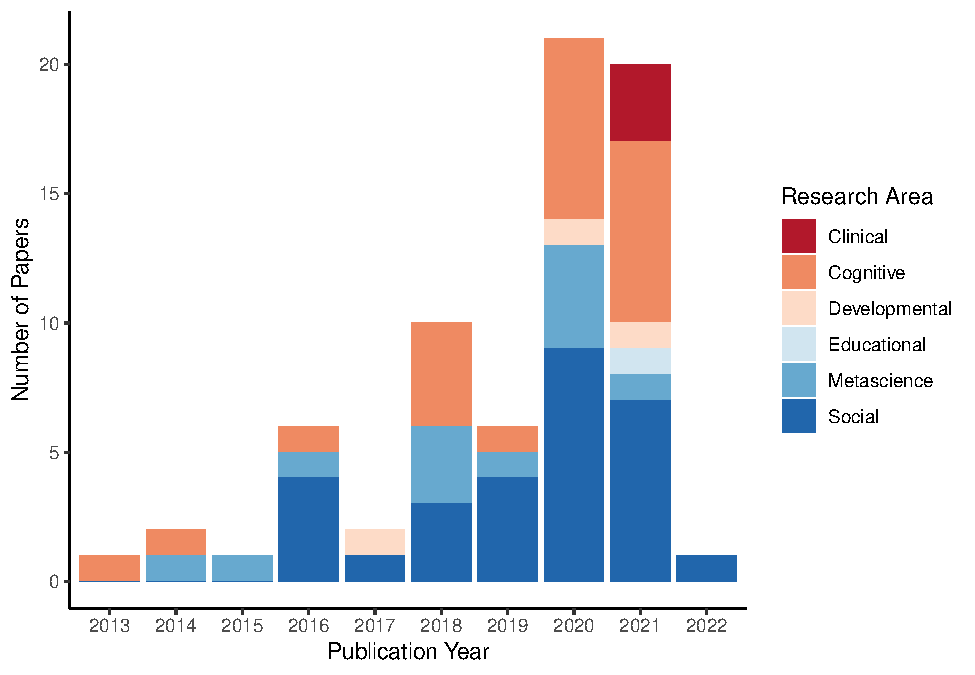
\includegraphics{04.manuscript_files/figure-latex/figure1-1.pdf}

\hypertarget{rq3-authors.-1}{%
\subsubsection{\texorpdfstring{RQ3: Authors.\\
}{RQ3: Authors. }}\label{rq3-authors.-1}}

\textbf{\emph{Career Length}}. The average career length was 11.97 (\emph{SD} = 7.95) for ORCID first publication year (i.e., current year minus year of first publication), \emph{M} = 13.12 (\emph{SD} = 8.74) for Scholar year of first publication, and \emph{M} = 13.54 (\emph{SD} = 7.77) for ORCID year of first degree. In each of the analyses, we use the actual year of first publication/education, as subtracting publication and using it as a predictor would create a perfect solution for each model.

Next, we will talk about the results from three variables:

\begin{enumerate}
\def\labelenumi{\arabic{enumi})}
\tightlist
\item
  ORCID year first publication:
\end{enumerate}

\begin{itemize}
\tightlist
\item
  The slope for year of first publication was \emph{b} = 0.00, \emph{SE} = 0.00, \emph{t}(53) = 1.71, \emph{p} = .092.
\item
  The variance parameter was \(SD\) = 7.99.
\item
  The slope for variance across years was \emph{b} = 0.01, \emph{SE} = 0.48, \emph{t}(23) = 0.02, \emph{p} = .983.
\end{itemize}

\begin{enumerate}
\def\labelenumi{\arabic{enumi})}
\setcounter{enumi}{1}
\tightlist
\item
  Scholar year first publication:
\end{enumerate}

\begin{itemize}
\tightlist
\item
  The slope for year of first publication was \emph{b} = 0.00, \emph{SE} = 0.00, \emph{t}(15) = 1.59, \emph{p} = .132.
\item
  The variance parameter was \(SD\) = 8.88.
\item
  The slope for variance across years was \emph{b} = 0.16, \emph{SE} = 0.61, \emph{t}(2) = 0.26, \emph{p} = .821.
\end{itemize}

\begin{enumerate}
\def\labelenumi{\arabic{enumi})}
\setcounter{enumi}{2}
\tightlist
\item
  ORCID year first degree:
\end{enumerate}

\begin{itemize}
\tightlist
\item
  The slope for year of first degree was \emph{b} = 0.00, \emph{SE} = 0.00, \emph{t}(35) = 5.14, \emph{p} = \textless{} .001.
\item
  The variance parameter was \(SD\) = 7.77.
\item
  The slope for variance across years was \emph{b} = 0.03, \emph{SE} = 0.82, \emph{t}(14) = 0.04, \emph{p} = .971.
\end{itemize}

Then we will discuss how these results are represented in our graph (below). We will discuss any discrepancies in the results across the three different statistics. We shall also make this graph more readable!

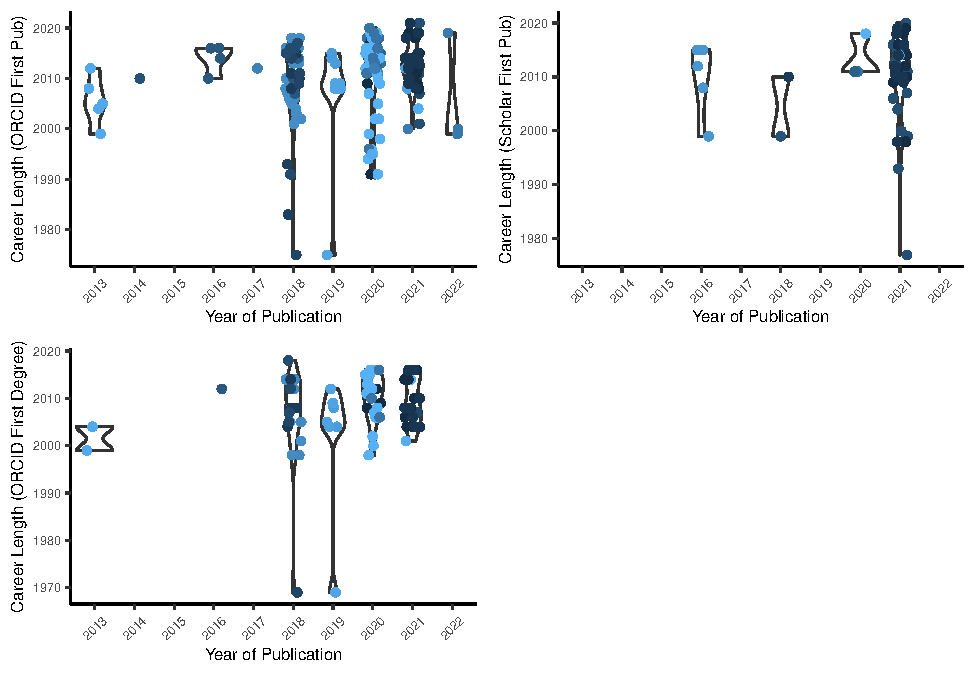
\includegraphics{04.manuscript_files/figure-latex/figure2-1.pdf}

\hypertarget{discussion}{%
\section{Discussion}\label{discussion}}

To be included after we have completed analyses.

\newpage

\hypertarget{references}{%
\section{References}\label{references}}

\begingroup
\setlength{\parindent}{-0.5in}
\setlength{\leftskip}{0.5in}

\hypertarget{refs}{}
\begin{CSLReferences}{0}{0}
\end{CSLReferences}

\endgroup


\end{document}
